\documentclass[12pt]{book}
\setlength{\headheight}{15pt}

\usepackage[margin=1in]{geometry}
\usepackage{color, colortbl}
\usepackage{fancyhdr}
\usepackage{amssymb}
\usepackage{amsmath}
\usepackage{lastpage}
\usepackage{karnaugh-map}
\usepackage{multicol}
\usepackage{multirow}
\usepackage{graphicx}

\graphicspath{ {./graphics/} }

% begin custom header shit
\pagestyle{fancy}
\fancyhf{}
\lhead{COMP2650 Lecture 12 - Sequential Logic I}
\rhead{Isaac Kilbourne (110043640)}
\rfoot{Page \thepage\ of \pageref{LastPage}}
% end custom header shit

\definecolor{LightRed}{rgb}{1, 0.6, 0.6}
\definecolor{LightGreen}{rgb}{0.6, 1, 0.6}
\newcolumntype{R}{>{\columncolor{LightRed}}c}
\newcolumntype{G}{>{\columncolor{LightGreen}}c}

\newenvironment{indented} {
	\begin{list}{}{\setlength{\leftmargin}{5mm}}
	\item[]
}{\end{list}}
	
\raggedbottom 
\begin{document}
    \noindent
    6.Design JK flip-flop using gated JKs (latches).
    \begin{indented}
        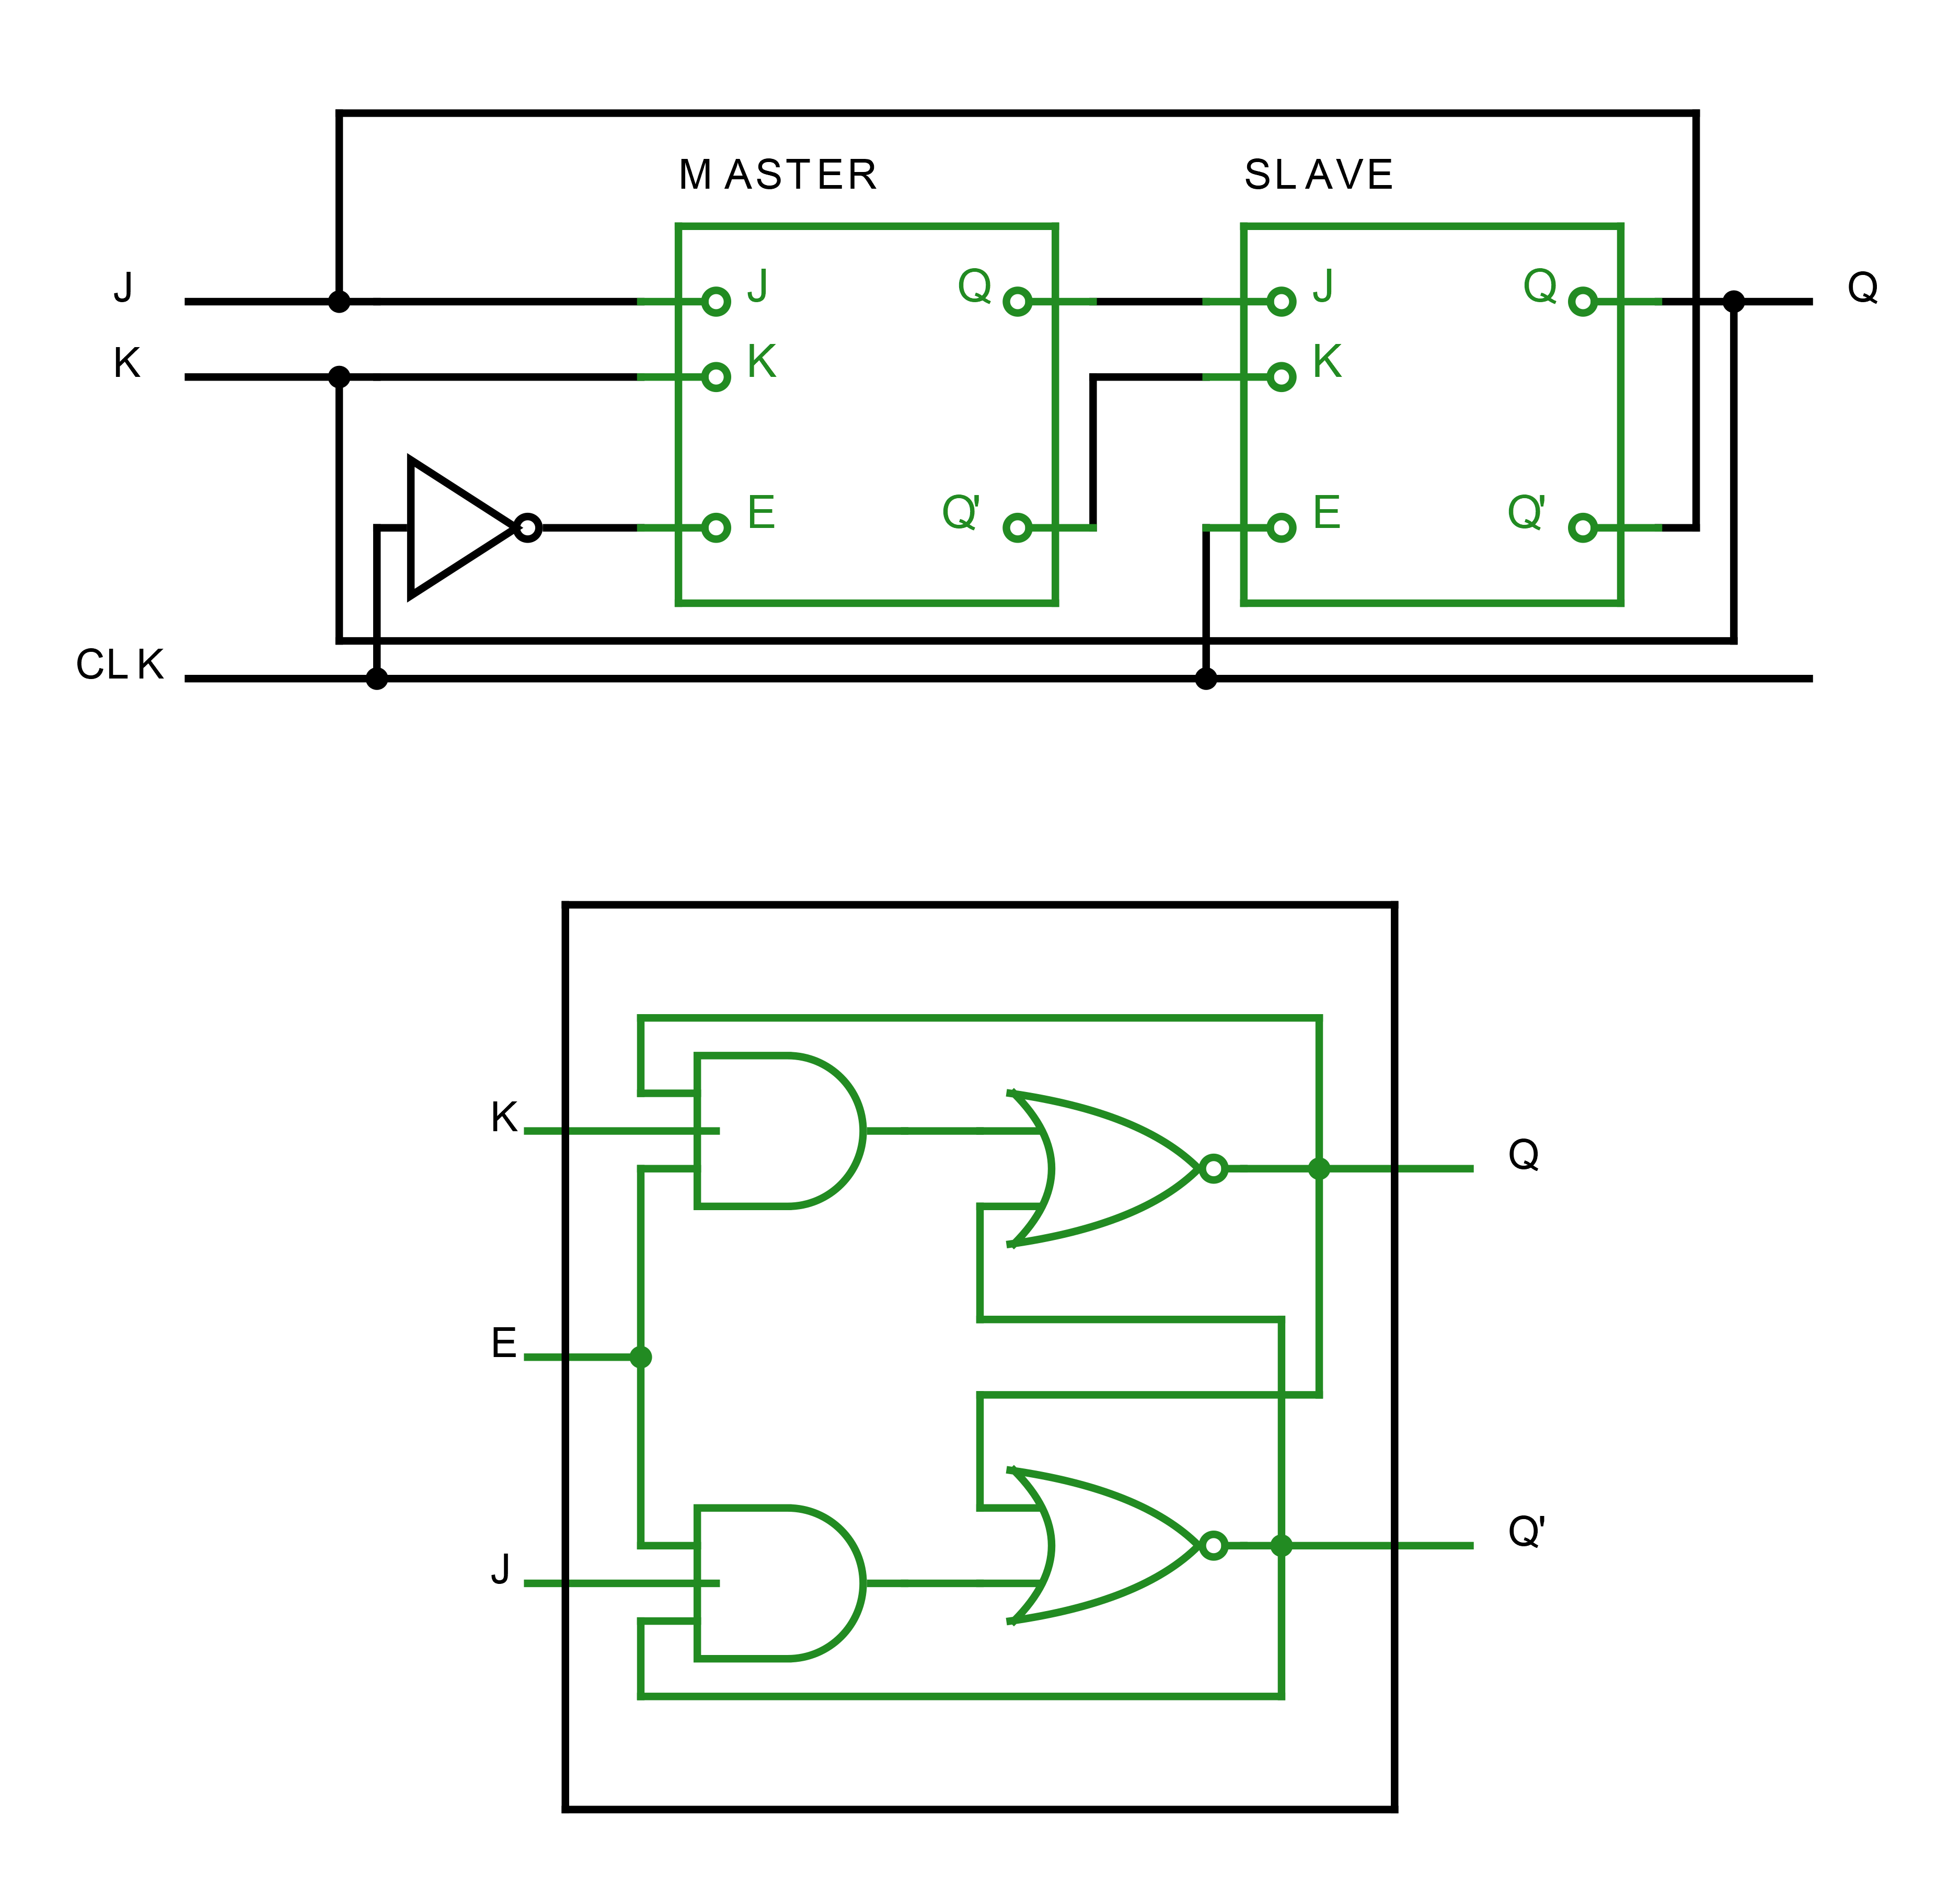
\includegraphics{q6_jk_ff}
    \end{indented}
    \vfill
    \footnotetext{I wasn't sure if a block diagram was acceptable or not, so the bottom circuit
    shows the inside of each of the JK latches. Additionally, I was unsure if the flip-flop
    should be rising, falling, or dual edge, so I designed it to be rising edge.}

    \pagebreak

    \noindent
    7.Design SR flip-flop using gated SRs (latches).
    \begin{indented}
        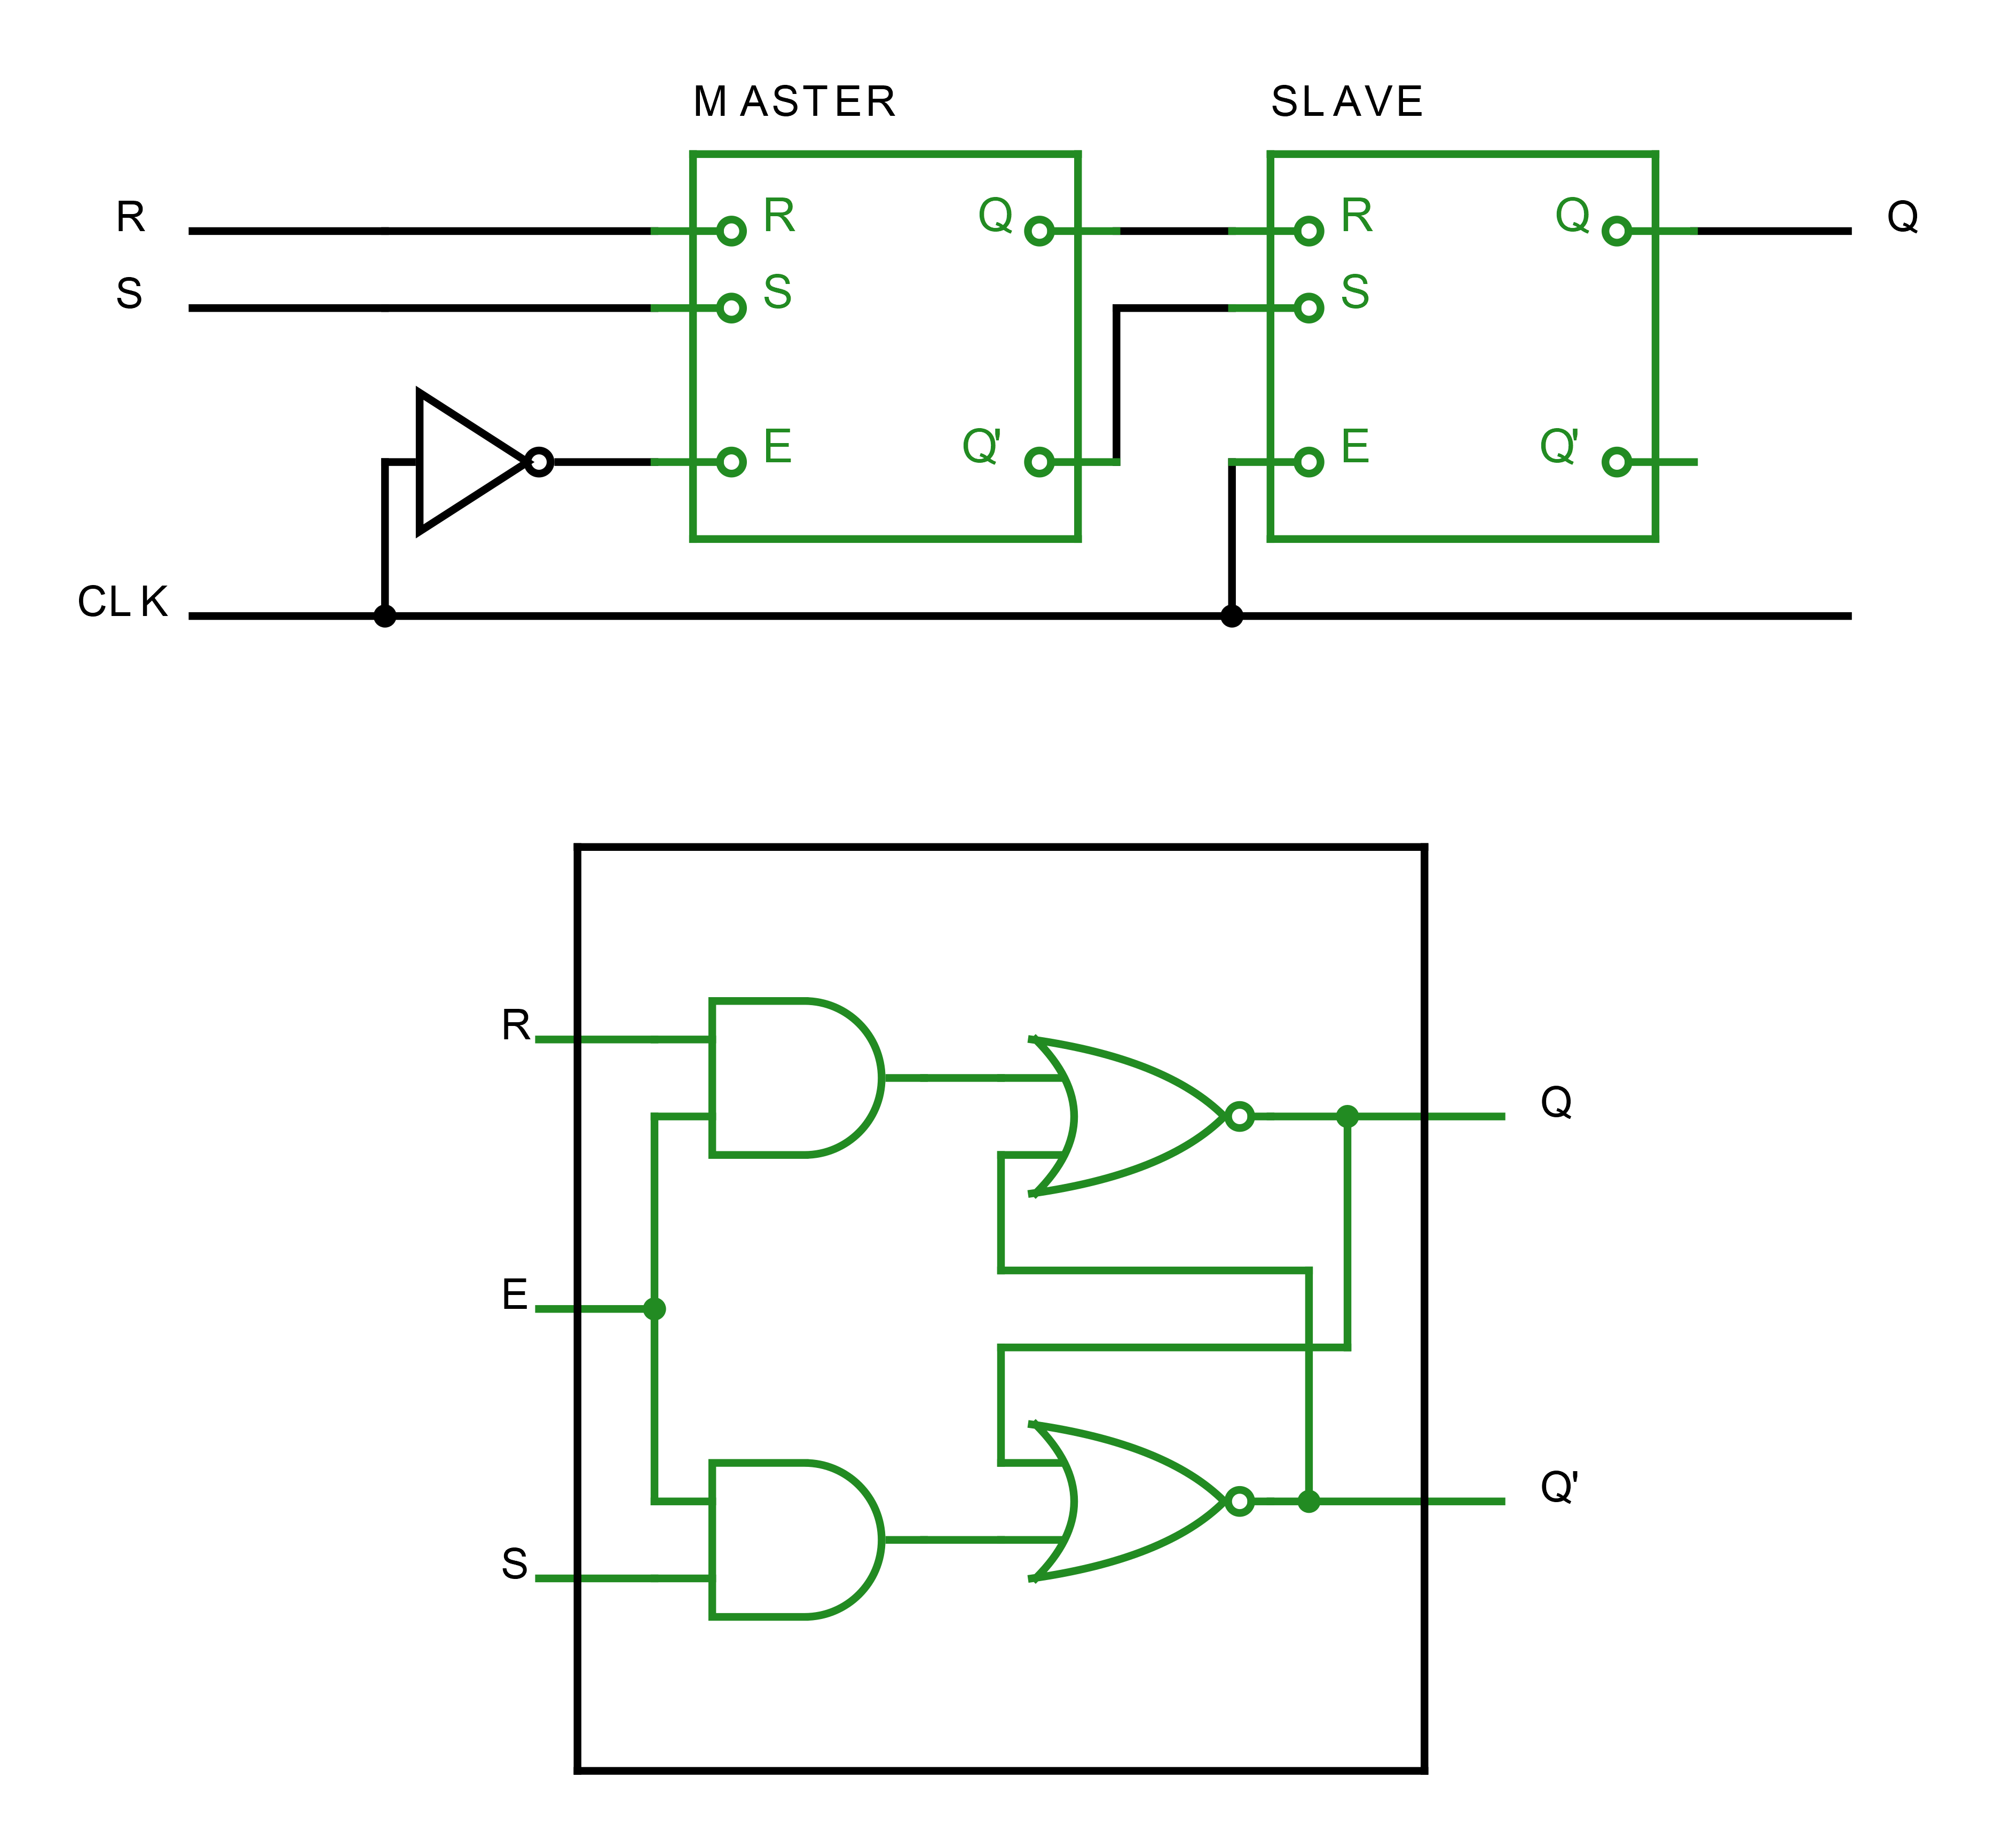
\includegraphics{q7_rs_ff.png}
    \end{indented}
    \vfill
    \footnotetext{Again, unsure about block diagrams so I made a compromise. This is also a 
    rising edge circuit since the instructions were vague.}
\end{document}
		